\begin{savequote}[8cm]
\textlatin{Neque porro quisquam est qui dolorem ipsum quia dolor sit amet, consectetur, adipisci velit...}

There is no one who loves pain itself, who seeks after it and wants to have it, simply because it is pain...
  \qauthor{--- Cicero's \textit{de Finibus Bonorum et Malorum}}
\end{savequote}

\chapter{\label{ch:hnl}HNL} 

\minitoc

    \section{Background}
        As a detailed review of HNL would exceed the scope of this report, only a highly simplified introduction to HNL is given here. 
        The origin of the neutrino mass is still a mystery. 
        One intuitive solution is to extend the neutrino family to include heavy members, which mix with the existing SM neutrinos via an extended PMNS matrix and give them the small masses observed via the see-saw mechanism~\cite{Abada:2007ux}. 
        As they mix the SM neutrinos, they could be produced in the intense neutrino beam in the long-baseline neutrino experiments, so the near detector of these experiments is the best place to look for HNL. 
        The signal comes from HNL decays, some of which are distinct from SM neutrino interactions. 
        Previously, T2K has searched for HNL~\cite{T2K:2019jwa} using the TPCs, a combined volume of about $7~\textrm{m}^3$, in ND280. As 
        the ND280 upgrade replaces the P0D with SFGD and HATPC, a combined volume of $8~\textrm{m}^3$, which are much better trackers than the P0D, they could be used in an HNL search as well, thereby improving the overall sensitivity. 

        To perform such an HNL search, a complicated chain of simulations is required, including the generation of an HNL flux based on the SM neutrino flux, the propagation of HNL and the decay of HNL. 
        The previous T2K search was based on a dedicated tool-set, \code{nd280HNLSim}, which was built only to search for $N\rightarrow l + \pi$ decay channels, where $l$ is a lepton. 
        It would require a large amount of efforts to extend it to include other production and decay channels. 
        Hence, I adapt the recently published general HNL package, \code{BeamHNL}~\cite{Plows:2022gxc}, to the T2K ND280 simulation to evaluate the sensitivity improvement brought by the upgrade.

    \section{Implementation}
        The simulation of HNL production and decay using \code{BeamHNL} is performed in several steps.
        Since \code{BeamHNL} is designed to be a cross-experiment package, it requires a standardized flux input in the \code{dk2nu} format. 
        The \code{dk2nu} file is a simple flat-tree ROOT file that must contain the minimally sufficient information for \code{BeamHNL} to function correctly.
        As the T2K flux is available in its specific format, a conversion is necessary. 
        The required \code{dk2nu} variables and the corresponding conversion from variables in a T2K flux file are provided in Appendix~\ref{sec:app-hnl-dk2nu}.

        Using this input, the desired HNL production channels can be performed by specifying a few additional parameters in a configuration \code{xml} file, \code{CommonHNL.xml}, located within the \code{GENIE} configuration directory. 
        These parameters are experiment-specific and must be set by the user. Details on how each parameter is set specifically for the T2K ND upgrade are provided in Appendix~\ref{sec:app-hnl-input}. 

        Before proceeding to subsequent steps, we validate the setup by feeding the T2K \code{dk2nu} file to \code{BeamHNL} and setting the HNL mass, $\mn$, to a small value, such as $1~\kev$. The output HNL flux should closely mimic the SM flux. 
        The result is shown in Fig.~\ref{fig:hnl-fluxes}, where the pink dashed line ($\mn=1~\kev$) closely overlaps with the black solid line, which is directly plotted from the T2K input flux.  
        \begin{figure}[!htb] 
            \centering 		
            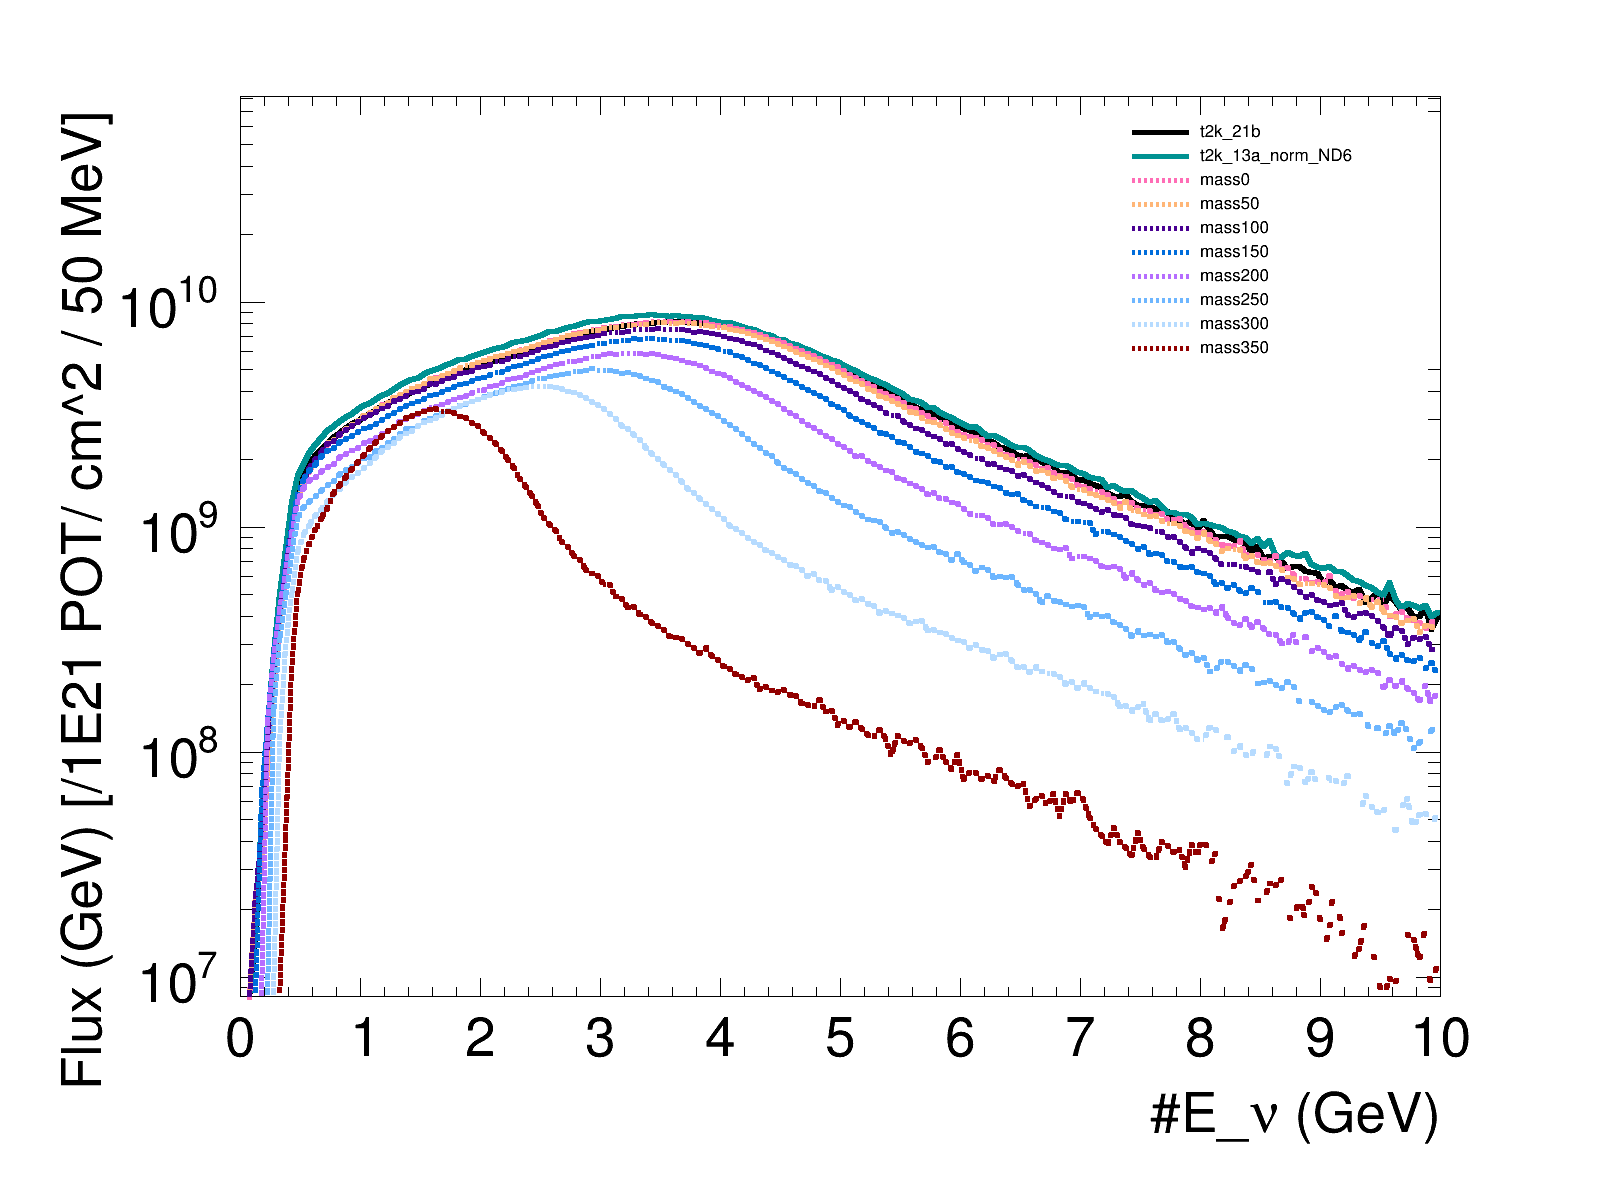
\includegraphics[width=\sgfigwid\textwidth]{figures/hnl_fluxes.png}
            \caption{\label{fig:hnl-fluxes} HNL fluxes produced by \code{BeamHNL} for different $M_N$. The solid lines are directly plotted from T2K input flux files, one with version ``13a'' and another with ``21b''. The dashed lines are \code{BeamHNL} outputs for different $\mn$.} 
        \end{figure}
        After validation, the HNL mass is set to target values, e.g., $300~\mev$, to generate HNL events, which are then passed through the T2K simulation chain for selection development. 
        \begin{figure}[!htb] 
            \centering 		
            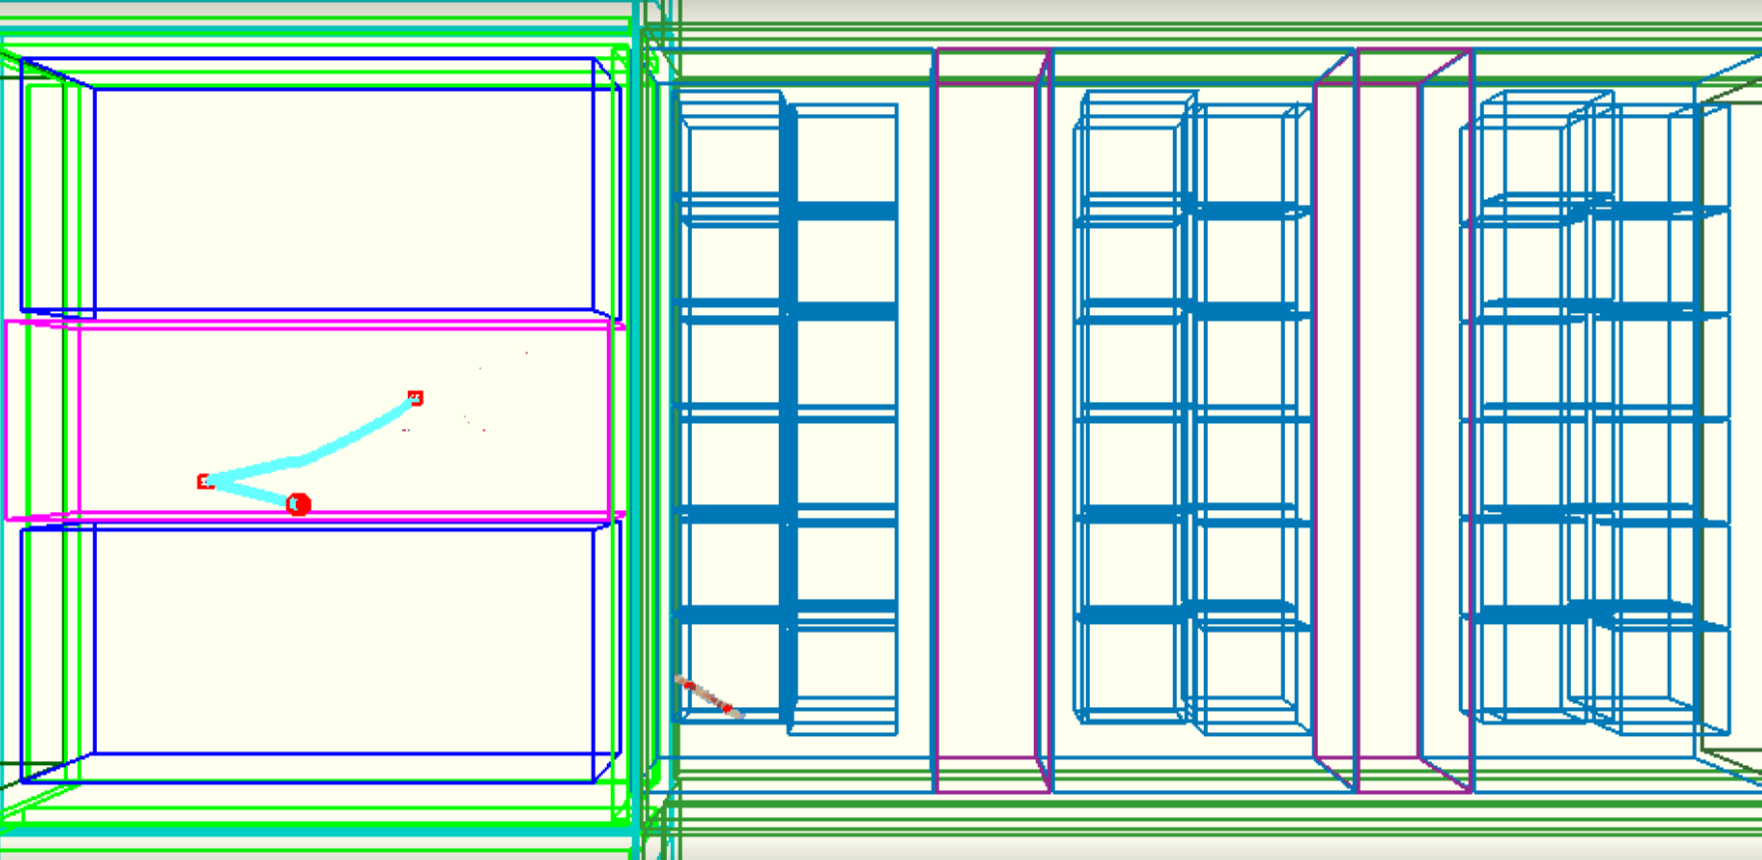
\includegraphics[width=\sgfigwid\textwidth]{figures/HNLEveDIs.png}
            \caption{\label{fig:hnl-evedis} A $N\rightarrow\mu+\pi$ event display in the upgraded ND280.} 
        \end{figure}

        It is logical to begin by developing a selection for the same signal channel as the previous T2K search to cross-validate before extending to additional channels. Therefore, I first developed the selection for the $N\rightarrow\mu+\pi$ channel. The steps are as follows:

        \begin{enumerate}
            \item \textbf{Basic T2K Event Quality Checks} 
            \item \textbf{Find SFGD Primary Vertex} 
            \item \textbf{Primary Track Count Cut} 
            \item \textbf{Escaping Muon Cut} 
            \item \textbf{Single Trackless Pion Cut}
            \item \textbf{Kink Cut}
            \item \textbf{$\mu$-$\pi$ Angle and Invariant Mass Cut}
            \item \textbf{$\mu$-$\pi$ $\dpt$ Cut}
        \end{enumerate}

        \textbf{Basic T2K Event Quality Checks} - A quality check ensures the event contains at least one reconstructed track.

        \textbf{Find SFGD Primary Vertex} - Identify a primary vertex in the SFGD. 
        Since the primary vertex for an HNL event does not necessarily include a muon, as in the $\numucc$ selection, the primary vertex should be identified independently from the primary muon. 
        All vertices are iterated through to record the number of tracks connected to each vertex, $n_{ptrk}$, and the length of the longest track connected to each vertex, $L_{max}$. 
        The vertex with the longest $L_{max}$ is selected as the primary vertex. 
        If more than one such vertex exists, the vertex with the largest $n_{trk}$ is selected. 
        If there is still more than one vertex, the vertex with the earliest time is selected.

        \textbf{Primary Track Count Cut} - For the target channel $N\rightarrow\mu+\pi$, there should be at most two primary tracks. Therefore, events with $n_{ptrk}>2$ are rejected.

        \textbf{Escaping Muon Cut} - This step identifies muons that escape the SFGD.

        \textbf{Single Trackless Pion Cut} and \textbf{Kink Cut} - These cuts are identical to those in the $\numuccopi$-Trackless selection, selecting a primary pion that has not undergone secondary interactions to ensure accurate reconstruction of its kinematics.

        \textbf{$\mu$-$\pi$ Angle and Invariant Mass Cut} - These are kinematic cuts that exploit the fact that SM events with one muon and one pion are mostly resonance events that have one more proton than HNL decays. Due to the additional proton, the opening angle between the $\mu$ track and the $\pi$ track, $\tmupi$, can vary widely, whereas in HNL decays, the angle is more collimated. Similarly, the invariant mass of the $\mu$-$\pi$ system, $\mmupi=(\pmu+\ppi)^2$, has a larger range compared to the HNL, which centers around the input value of $300~\mev$, as shown in Fig.~\ref{fig:hnl-mmupi}.
        The stark contrast is apparent in Fig.~\ref{fig:mmupi-mupiang}. To preserve the largest number of HNL events, the specific cuts applied are: $30\deg < \tmupi < 90\deg$ and $270~\mev<\mmupi<320~\mev$. 
        \begin{figure}[!htb]
           \centering
           \begin{subfigure}{\dbfigwid\textwidth}
                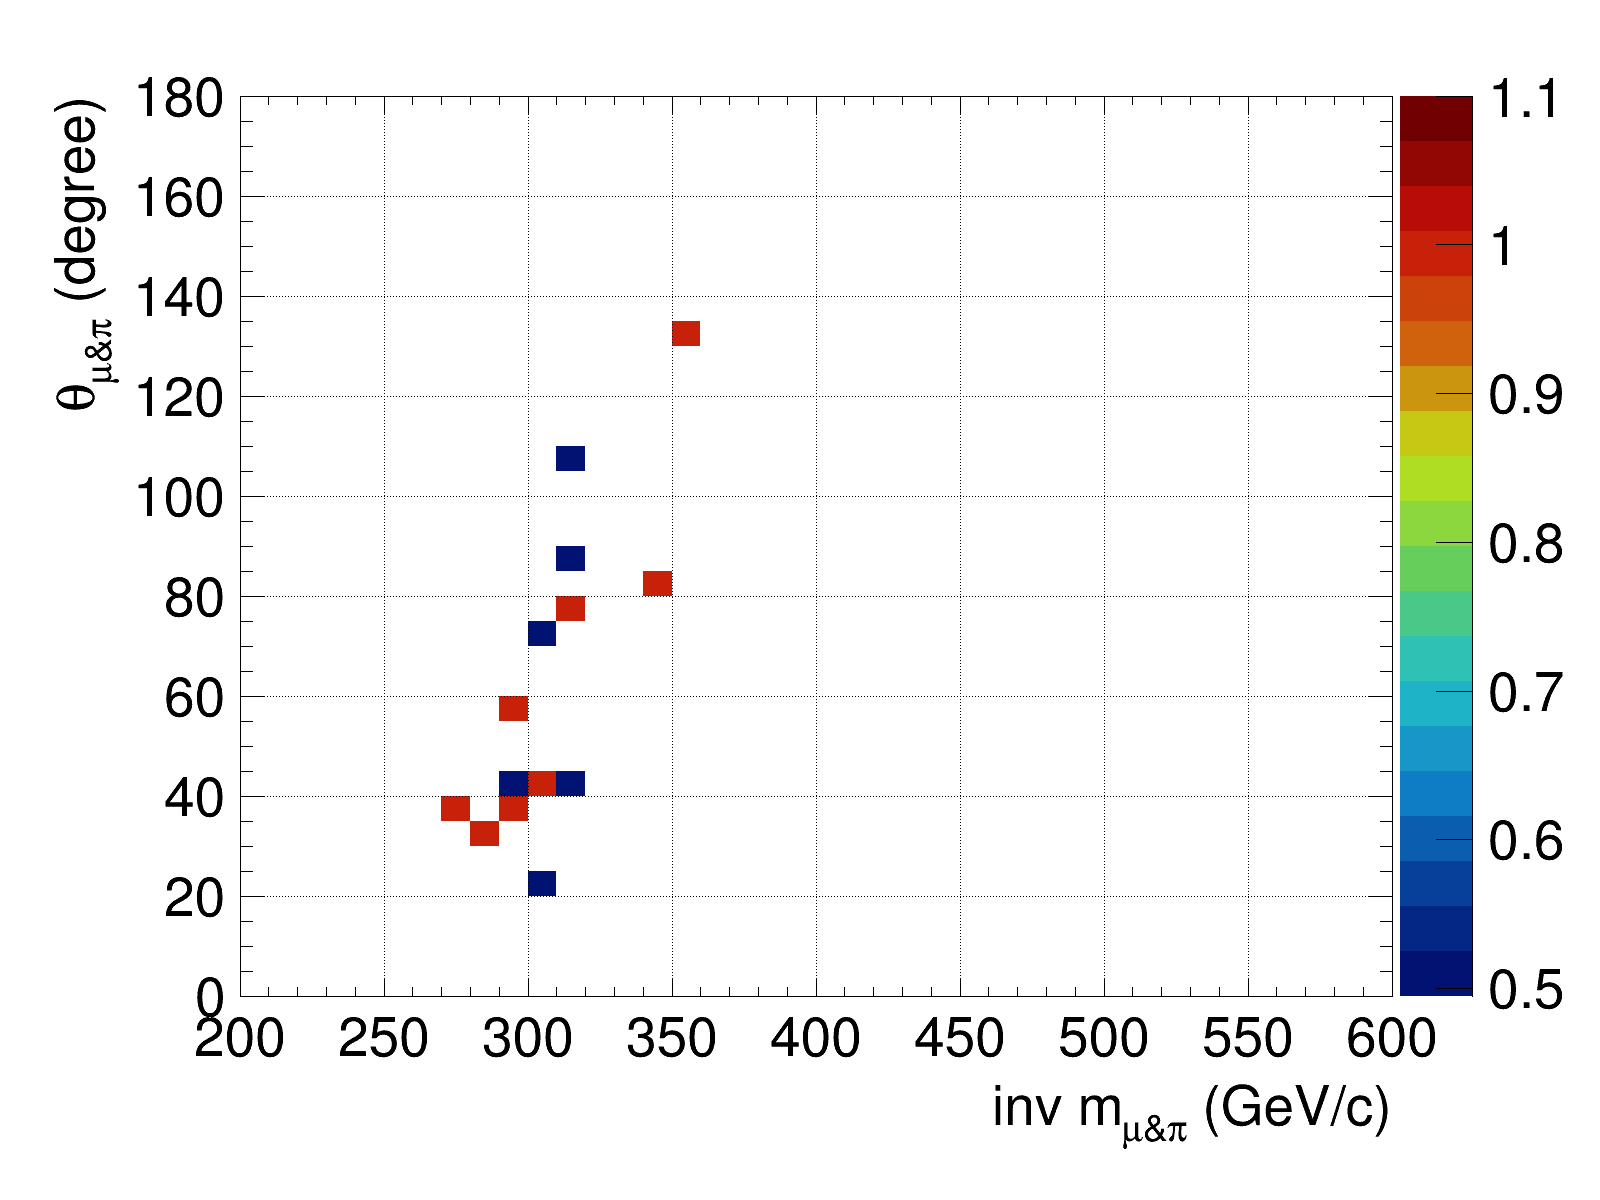
\includegraphics[width=\textwidth]{figures/hnl_sfgmu_mpinvm_colnor_vs_mpang_hist2d_al9_300.png}
                \caption{HNL.}
                \label{fig:hnl-mmupi}
           \end{subfigure}
           \begin{subfigure}{\dbfigwid\textwidth}
                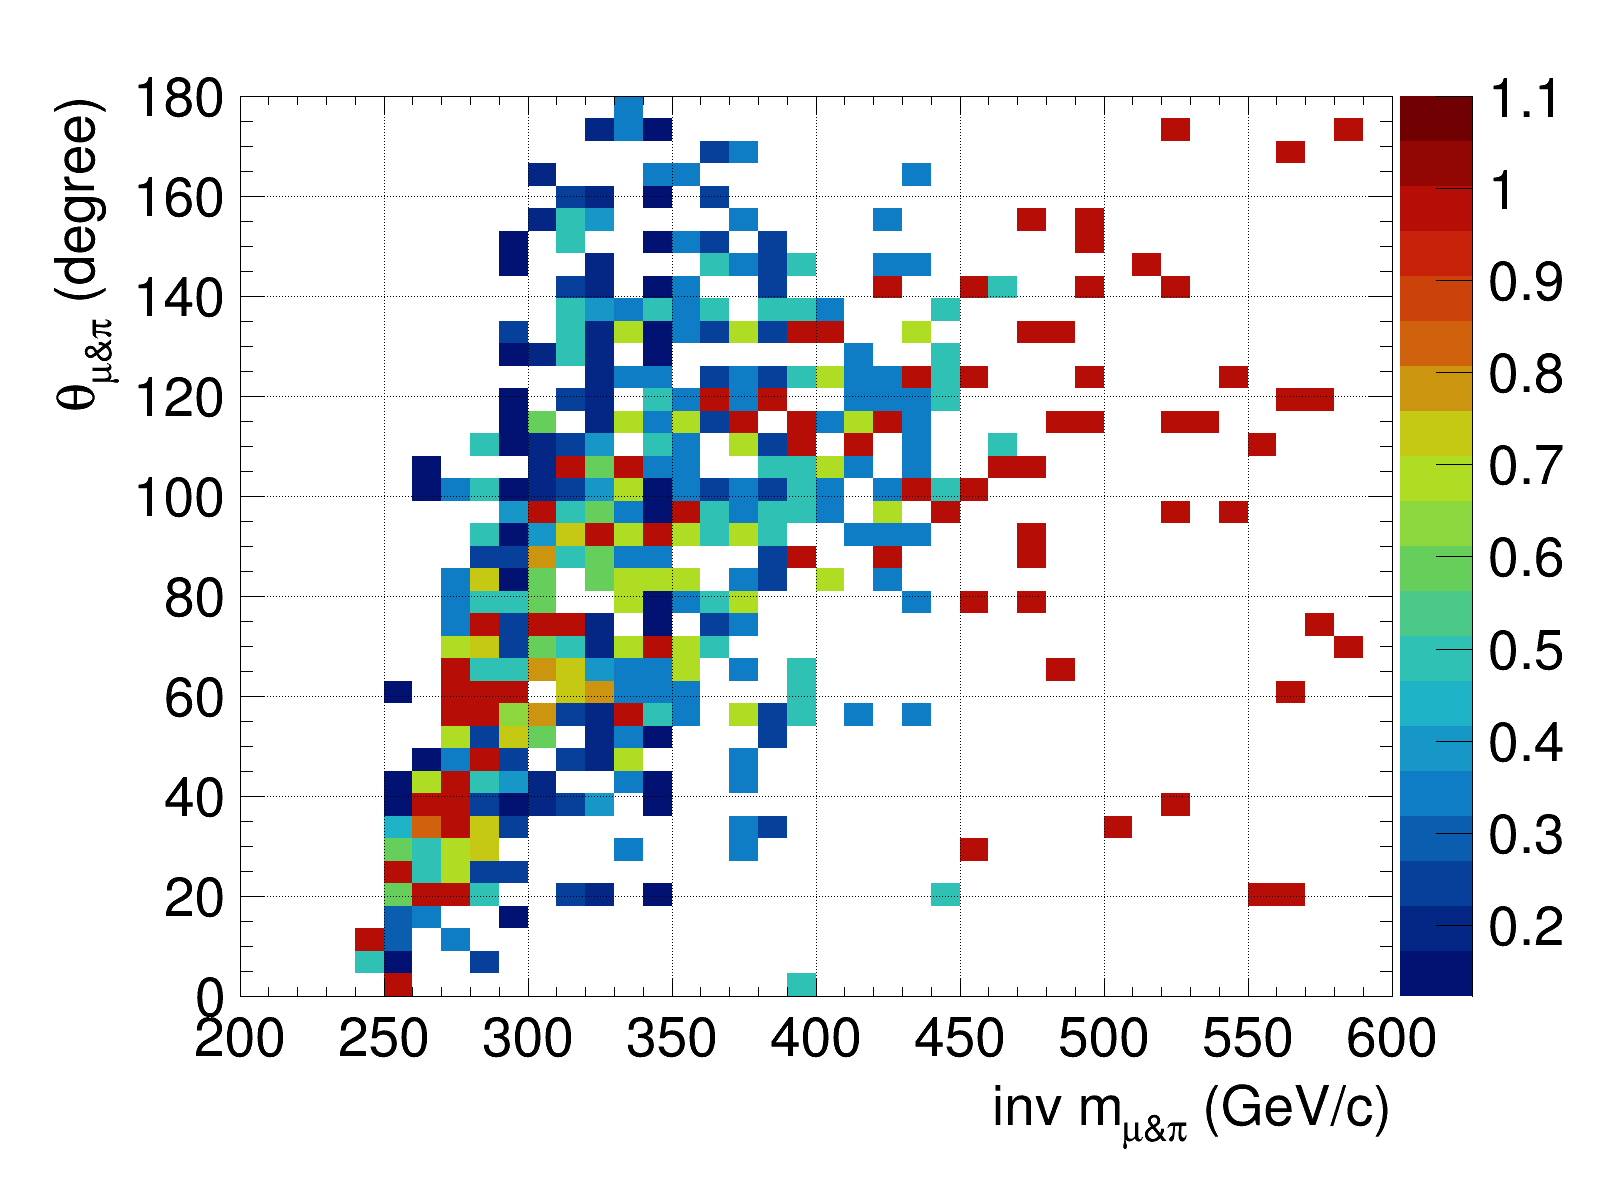
\includegraphics[width=\textwidth]{figures/hnl_sfgmu_mpinvm_colnor_vs_mpang_hist2d_al9_SM.png}
                \caption{SM $\nu$.}
                \label{fig:sm-mmupi}
           \end{subfigure}
           \caption{$\tmupi$ plotted against $\mmupi$.}
           \label{fig:mmupi-mupiang}
        \end{figure}

        \textbf{$\mu$-$\pi$ $\dpt$ Cut} - Similar to previous kinematic cuts, the net transverse momentum of $\mu$ and $\pi$ should be small, while for SM events it has a much larger range, as shown in Fig.~\ref{fig:mmupi-dpt}. By applying the cut $\dptmupi<15~\mevc$, eight HNL events survived with zero SM backgrounds.

        \begin{figure}[!htb]
           \centering
           \begin{subfigure}{0.45\textwidth}
                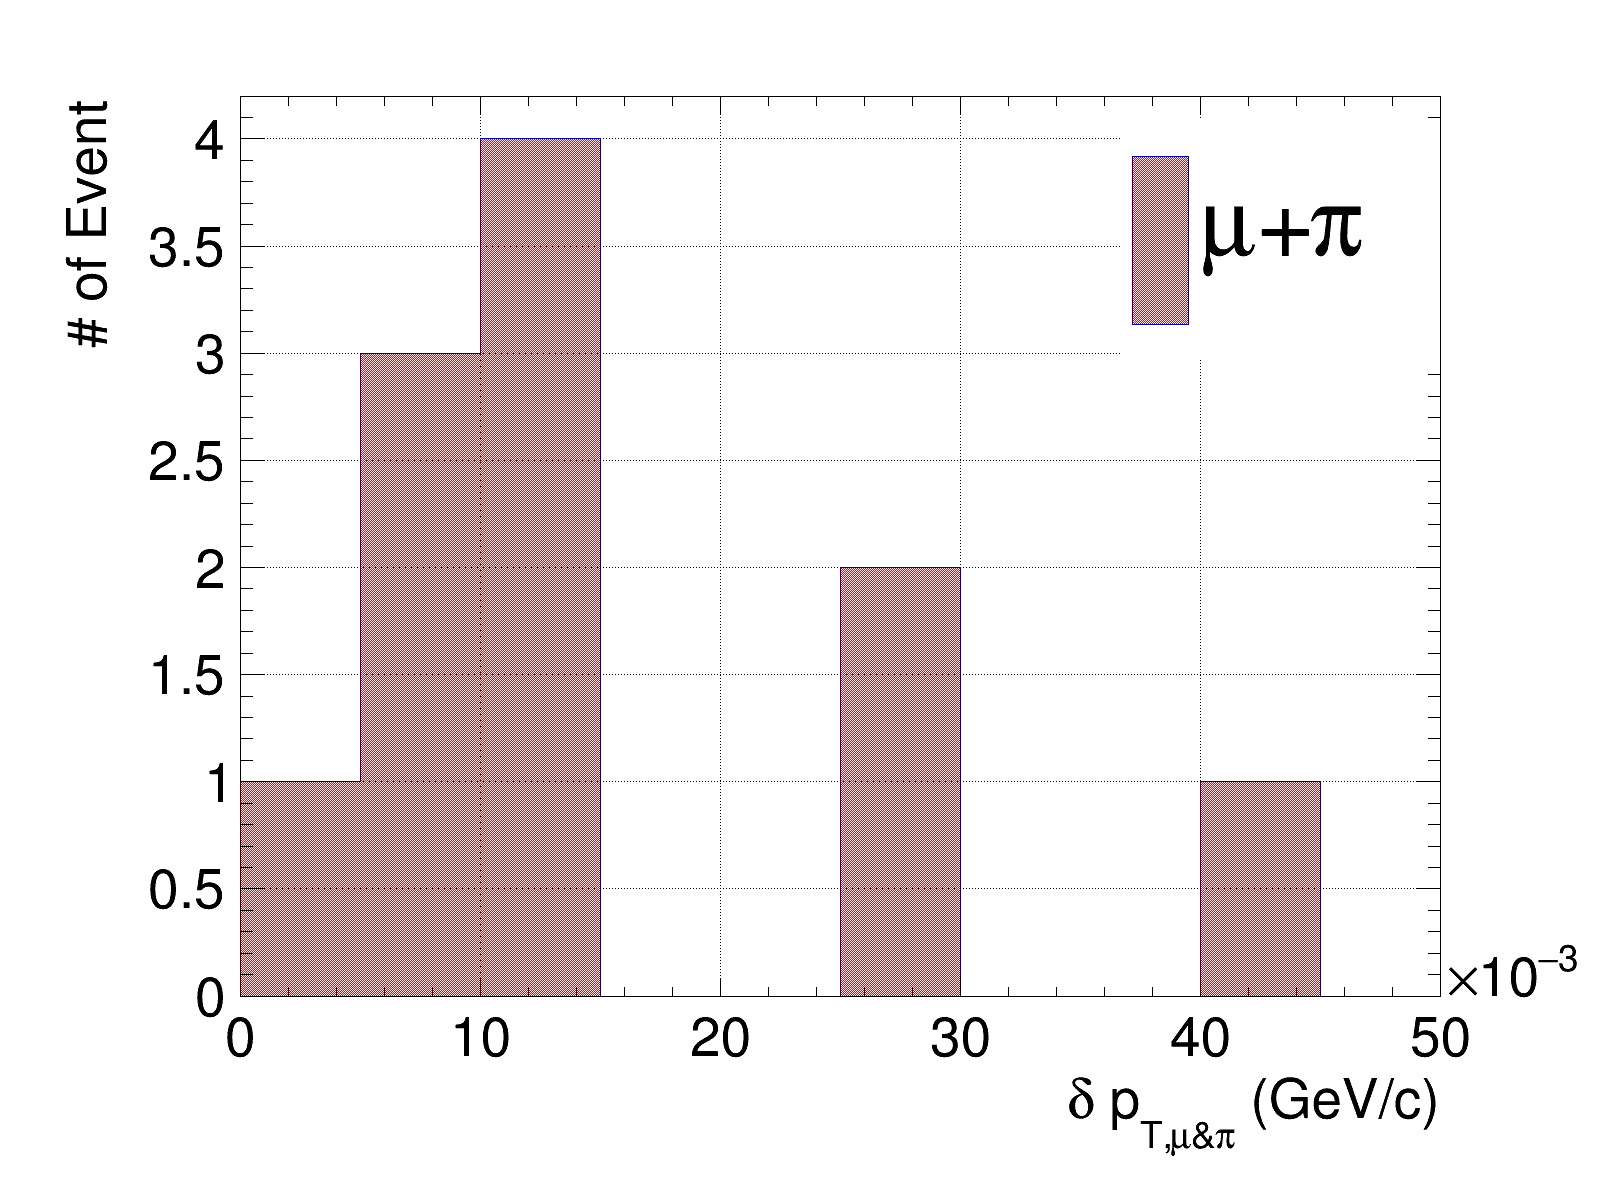
\includegraphics[width=\textwidth]{figures/hnl_sfgmu_mpdpt_stack_al9_300_aftmupikin.png}
                \caption{HNL.}
                \label{fig:hnl-mupidpt}
           \end{subfigure}
           \begin{subfigure}{0.45\textwidth}
                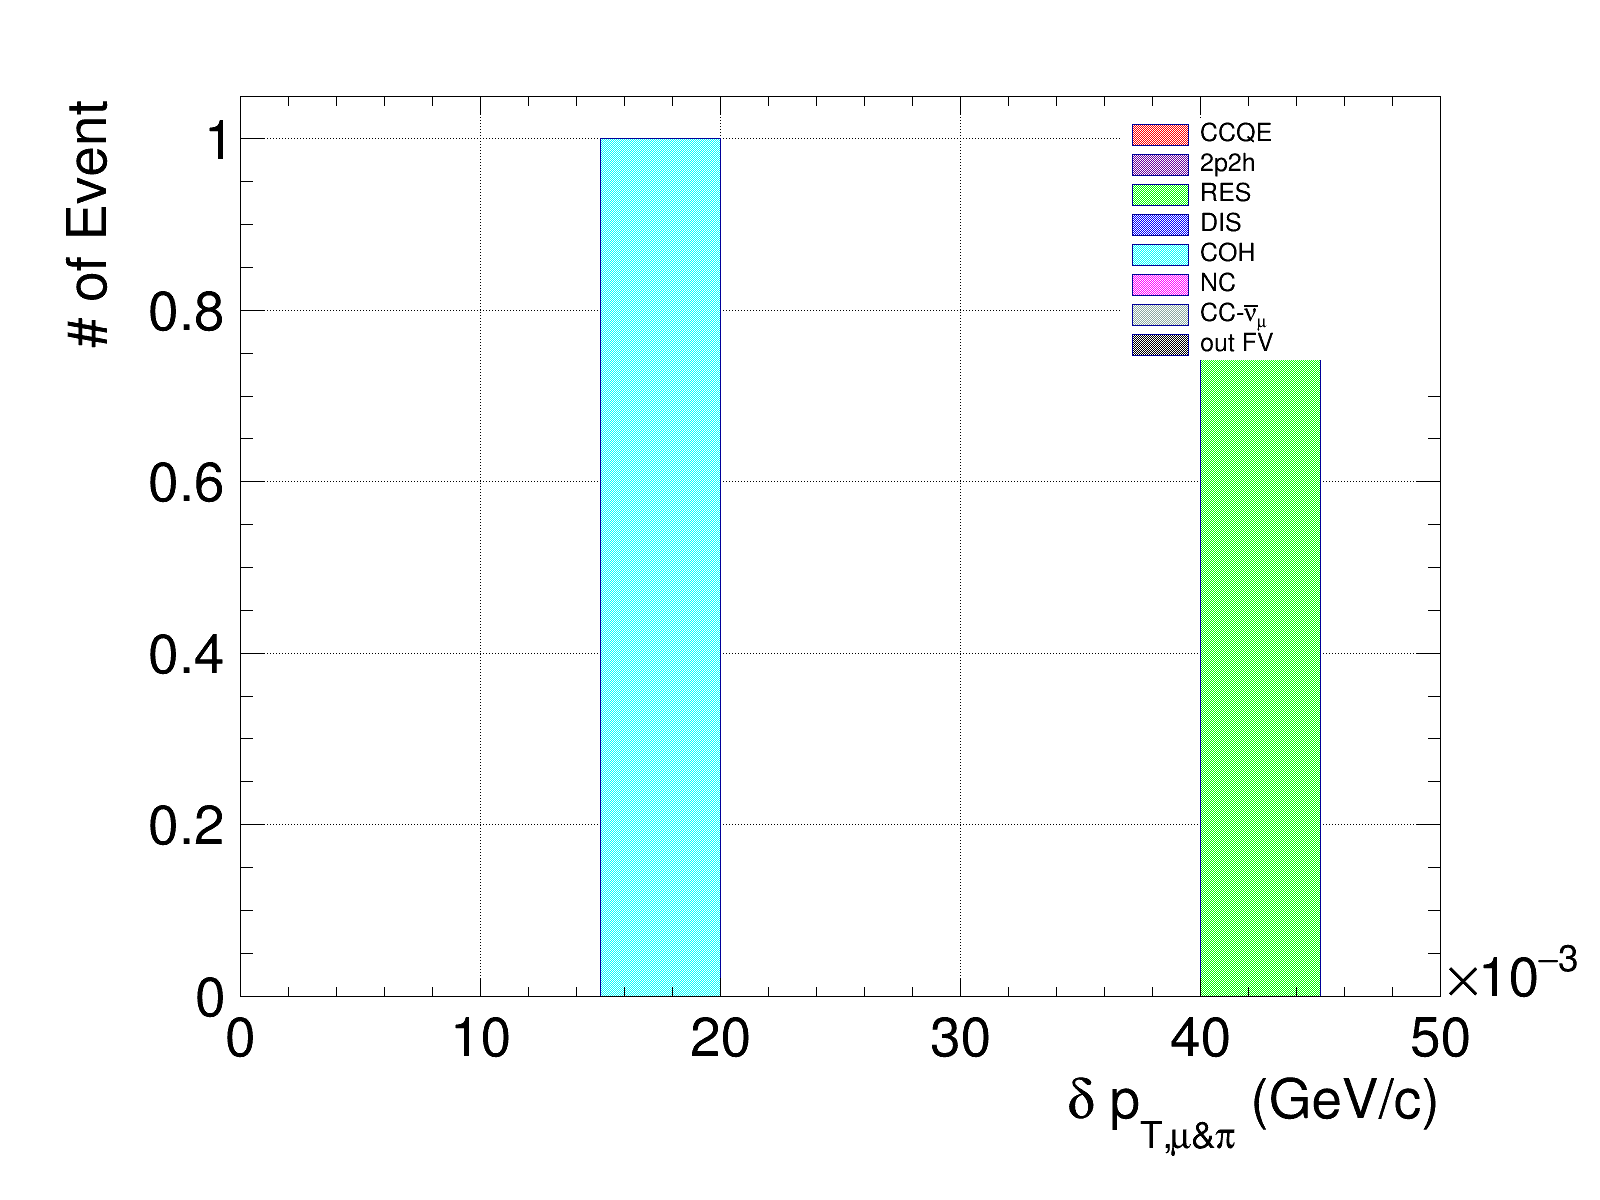
\includegraphics[width=\textwidth]{figures/hnl_sfgmu_mpdpt_stack_al9_SM_aftmupikin.png}
                \caption{SM $\nu$.}
                \label{fig:sm-mupidpt}
           \end{subfigure}
           \caption{$\dptmupi$ distributions for HNL and SM $\nv$.}
           \label{fig:mmupi-dpt}
        \end{figure}

    
    \section{Background estimation}
        A comprehensive background estimation is not yet complete; however, preliminary results from Fig.~\ref{fig:sm-mupidpt} suggest that coherent pion production is the dominant source. 
        From a crude estimation, as shown in Fig.~\ref{fig:coh-bkg}, the area under the fitted curve for $\dptmupi<15~\mevc$ is approximately $0.5$. 
        \begin{figure}[!htb] 
            \centering
            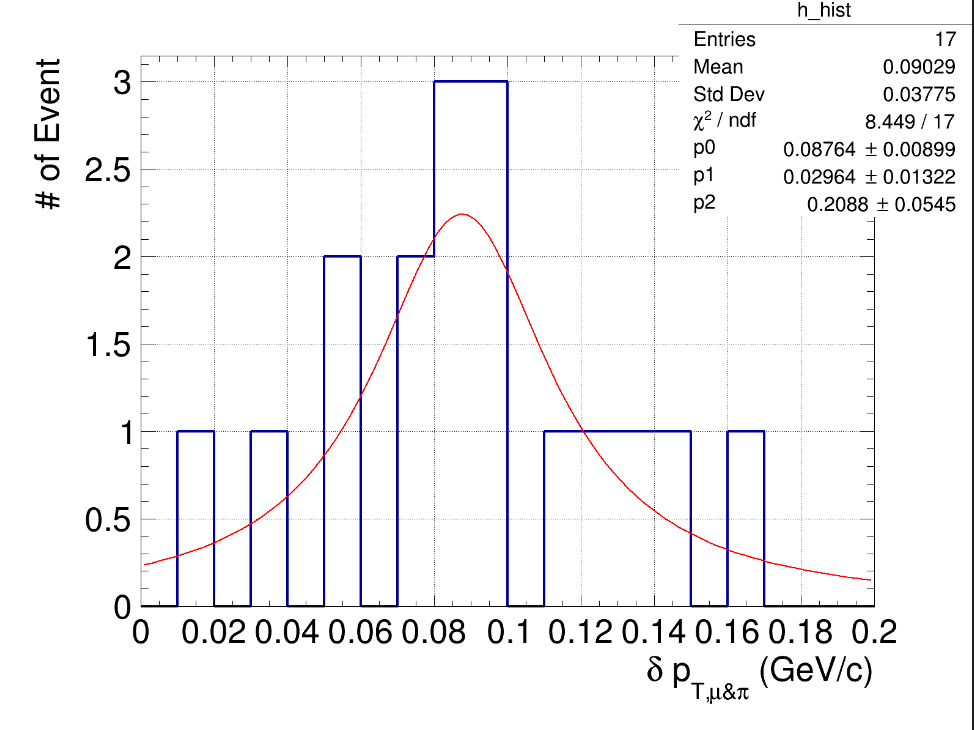
\includegraphics[width=0.5\linewidth]{figures/COH.png}
            \caption{Coherent background estimation. \blue{TO be re-plotted.}}
            \label{fig:coh-bkg}
        \end{figure}    
    
    \section{Sensitivity extraction}
        Sensitivity is extracted using the $CL_s$ method~\cite{Read:2002hq}.
        $CL_x$ is defined as $\textrm{Prob}(N\leq N_{\textrm{obs}}| \mu = x)$, i.e., the probability of predicting a number of events smaller than or equal to the number of observed events assuming model $x$. When $x=b$ or $x=s+b$, it corresponds to the background-only model or the signal plus background model, respectively.
        Then, $CL_s$ is defined as 
        \begin{equation}
            CL_s = \frac{CL_{s+b}}{CL_{b}} = \frac{\textrm{Prob}(N\leq N_{\textrm{obs}}| \mu = s+b)}{\textrm{Prob}(N\leq N_{\textrm{obs}}| \mu = b)} = \alpha,
        \end{equation}
        where $1-\alpha$ is the confidence level.

        For a target confidence level, $f$, one starts from $s=0$ and iterates with increasing $s$ to find the largest $s_{up}$ such that $\alpha < 1-f$. 
        Then, $s_{up}$ is the upper limit for the number of signal events at confidence level $f$ such that the background-only model is not rejected. 
        When a more detailed background model is available, it is conventional to use the median number of background events to evaluate $s_{up}$.
        A limit can then be placed on the mixing element $\umas$ based on its proportional relation to $s_{up}$.

        Specifically, in the above example, $100,000$ \genie events were simulated using \code{BeamHNL}. 
        The total number of protons on target (POT) required to produce these HNL events is calculated from \code{BeamHNL} output to be approximately $0.81\times10^{21}$ assuming $\umas=10^{-7}$. 
        Hence, we expect $8/0.81\approx9.9$ selected signals per $10^{21}$ POT.
        For this estimation, the background is taken to be $0.5$, and then $s_{up}$ is calculated to be $2.3$. 
        Hence, the limit on $\umas$ is calculated as 
        \begin{align}
            \left(\frac{U_{up}}{10^{-7}}\right)^2 & =  \frac{2.3}{9.9} \\
            U_{up} & = 10^{-7} \times \sqrt{\frac{2.3}{89}} = 4.8\times10^{-8}
        \end{align}

    \section{Discussion}
        This result is larger than the limit placed by the previous search, $U_{up}\approx4\times10^{-9}$, for $\mn=300~\mev$. 
        However, it is roughly of the same order of magnitude. 
        Moreover, the current result includes only events in SFGD, which has only about $1/3$ of the volume compared to the vertical TPCs. 
        Most importantly, this preliminary result demonstrates that SFGD can also provide excellent signal-background separation for HNL searches.
        Hence, it will definitely improve the limits by adding it to the existing search. 
        The next step is to extend the selection to the entire upgraded ND280 when the HAT reconstruction becomes available and to investigate the overall improvement in HNL sensitivity brought by the upgrade.